%%%%%%%%%%%%%%%%%%%%%%%%%%%%%%% document and size %%%%%%%%%%%%%%%%%%%%%%%%%%%%%%
\documentclass[10pt]{beamer}

%%%%%%%%%%%%%%%%%%%%%%%%%%%%% special libraries %%%%%%%%%%%%%%%%%%%%%%%%%%%%%%%%
\usepackage{ngerman}
\usepackage{tikz}
\usetikzlibrary{arrows,automata}
\usepackage{fancyhdr}
\usepackage[export]{adjustbox}
\usepackage{lipsum}
%%%%%%%%%%%%%%%%%%%%%%%%%%%%%% custum commands %%%%%%%%%%%%%%%%%%%%%%%%%%%%%%%%%
\newcommand{\gap}{\ \\ \ \\}
%%%%%%%%%%%%%%%%%%%%%%%%%%%%%%%%% DO NOT TOUCH %%%%%%%%%%%%%%%%%%%%%%%%%%%%%%%%%
\setbeamerfont{footnote}{size=\scriptsize}
\setbeamertemplate{footline}{}
\setbeamercolor{footnote}{fg=white,bg=mDarkTeal}


\usetheme[progressbar=frametitle]{metropolis}
\usepackage{appendixnumberbeamer}

\usepackage{booktabs}
\usepackage[scale=2]{ccicons}

\usepackage{pgfplots}
\usepgfplotslibrary{dateplot}

\usepackage{xspace}
\newcommand{\themename}{\textbf{\textsc{metropolis}}\xspace}

\title{Der Linearzeit MST Algorithmus}
\subtitle{Ein randomisierter Ansatz f"ur bessere Performanz}
\date{}
\author{Max Springenberg}
\institute{Proseminar: Randomisierte Algorithmen, TU Dortmund}
%%%%%%%%%%%%%%%%%%%%%%%%%%%%%%%%%%%%%%%%%%%%%%%%%%%%%%%%%%%%%%%%%%%%%%%%%%%%%%%%

\begin{document}

\maketitle
\begin{frame}{Table of contents}
  \setbeamertemplate{section in toc}[sections numbered]
  \tableofcontents[hideallsubsections]
\end{frame}

% MST
% * was ist ein MST
% * was ist ein minimaler MST
\section{MST in gewichteten Graphen}
\begin{frame}
    Ein Teilgraph $T$ ist genau dann ein minimaler Spannbaum von $G$, 
    wenn er alle Knoten verbindet und die Summe seiner Kantengewichte 
    $\underset{e \in E_T}{\sum} w(e)$ 
    minimal ist.\\
\end{frame}
\begin{frame}
    Ein Teilgraph $T$ ist genau dann ein minimaler Spannbaum von $G$, 
    wenn er alle Knoten verbindet und die Summe seiner Kantengewichte 
    $\underset{e \in E_T}{\sum} w(e)$
    minimal ist.\\
    \gap
    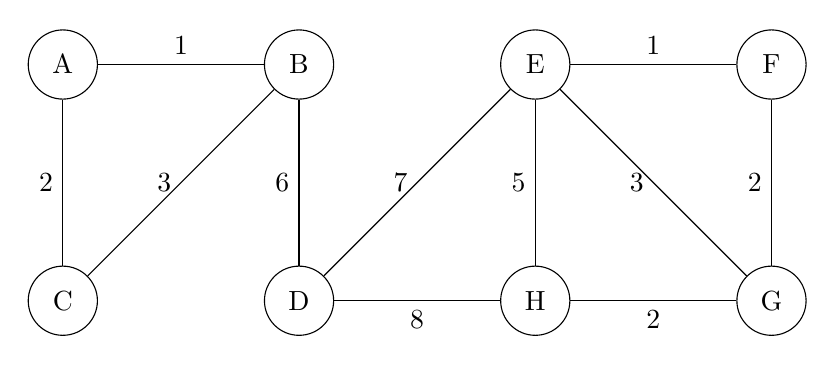
\begin{tikzpicture}
        \node[state](A) at (0,0)  {A};
        \node[state](B) at (3,0)  {B};
        \node[state](C) at (0,-3) {C};
        \node[state](D) at (3,-3) {D};
        \node[state](E) at (6,0)  {E};
        \node[state](F) at (9,0)  {F};
        \node[state](G) at (9,-3) {G};
        \node[state](H) at (6,-3) {H};
        \path
            (A) edge [-, above] node {1} (B)
                edge [-, left ] node {2} (C)
            (B)
                edge [-, left ] node {3} (C)
                edge [-, left ] node {6} (D)
            (D)
                edge [-, left ] node {7} (E)
                edge [-, below] node {8} (H)
            (E)
                edge [-, above] node {1} (F)
                edge [-, left ] node {3} (G)
                edge [-, left ] node {5} (H)
            (F)
                edge [-, left ] node {2} (G)
            (G)
                edge [-, below] node {2} (H)
            ;
    \end{tikzpicture}
\end{frame}
\begin{frame}
    Ein Teilgraph \textcolor{orange}{$T$} ist genau dann 
    ein \textcolor{orange}{minimaler Spannbaum} von $G$, 
    wenn er alle Knoten verbindet und die 
    Summe seiner Kantengewichte 
    \textcolor{orange}{$\underset{e \in E_T}{\sum} w(e)$ minimal} ist.\\
    \gap
    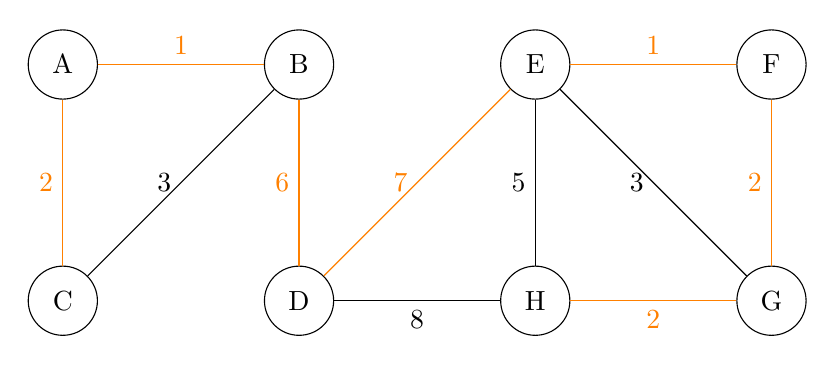
\begin{tikzpicture}
        \node[state](A) at (0,0)  {A};
        \node[state](B) at (3,0)  {B};
        \node[state](C) at (0,-3) {C};
        \node[state](D) at (3,-3) {D};
        \node[state](E) at (6,0)  {E};
        \node[state](F) at (9,0)  {F};
        \node[state](G) at (9,-3) {G};
        \node[state](H) at (6,-3) {H};
        \path
            (A) edge [-, above, color=orange] node {1} (B)
                edge [-, left , color=orange] node {2} (C)
            (B)
                edge [-, left ] node {3} (C)
                edge [-, left , color=orange] node {6} (D)
            (D)
                edge [-, left , color=orange] node {7} (E)
                edge [-, below] node {8} (H)
            (E)
                edge [-, above, color=orange] node {1} (F)
                edge [-, left ] node {3} (G)
                edge [-, left ] node {5} (H)
            (F)
                edge [-, left , color=orange] node {2} (G)
            (G)
                edge [-, below, color=orange] node {2} (H)
            ;
    \end{tikzpicture}
\end{frame}

% B"aume vs W"alder
% * Was ist ein Wald?
\section{B"aume vs. W"alder}

% Boruvka Phasen:
% * Wie werden zu kontraktierende Kanten ausgew"ahlt?
% * Was ist die Maximale Gr"o"se des Graphen nach einer Phase?
\section{Boruvka Phasen}
\begin{frame}
    \begin{tikzpicture}
    \end{tikzpicture}
\end{frame}
\begin{frame}{Ablauf}
    \begin{enumerate}
        \item Kontraktierende Kanten markieren
        \item Verbundene Komponente bestimmen
        \item Verbundene Komponenten durch einzelnen Knoten ersetzen
        \item Selbstschleifen entfernen
    \end{enumerate}
\end{frame}

% F-schwere/ leichte Kanten
% * wann ist eine Kante F-schwer
% * wann ist sie F-leicht
% * kann eine F-schwere Kante im MST enthalten sein?
\section{F-schwere/ leichte Kanten}

% Randomisierte Stichproben
% * `w"urfeln` erkl"aren
\section{Randomiserte Stichprobem}

% Wie k"onnen 
\begin{frame}
    Wirf eine M"unze!
    
\includegraphics{coin-flip-clipart.png}
\end{frame}

\begin{frame}
    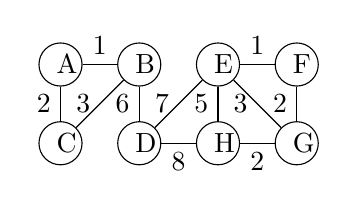
\begin{tikzpicture}[minND/.style={circle,
                                      draw=black,
                                      text width=1mm,
                                      inner sep=3pt,
                                      align=center,
                                      fill=white,
                                      text centered}]
        \node[minND](A) at (0,0)  {A};
        \node[minND](B) at (1,0)  {B};
        \node[minND](C) at (0,-1) {C};
        \node[minND](D) at (1,-1) {D};
        \node[minND](E) at (2,0)  {E};
        \node[minND](F) at (3,0)  {F};
        \node[minND](G) at (3,-1) {G};
        \node[minND](H) at (2,-1) {H};
        \path
            (A) edge [-, above] node {1} (B)
                edge [-, left ] node {2} (C)
            (B)
                edge [-, left ] node {3} (C)
                edge [-, left ] node {6} (D)
            (D)
                edge [-, left ] node {7} (E)
                edge [-, below] node {8} (H)
            (E)
                edge [-, above] node {1} (F)
                edge [-, left ] node {3} (G)
                edge [-, left ] node {5} (H)
            (F)
                edge [-, left ] node {2} (G)
            (G)
                edge [-, below] node {2} (H)
            ;
    \end{tikzpicture} \ \\
\end{frame}

\section{Erkenntnis}
\begin{frame}
    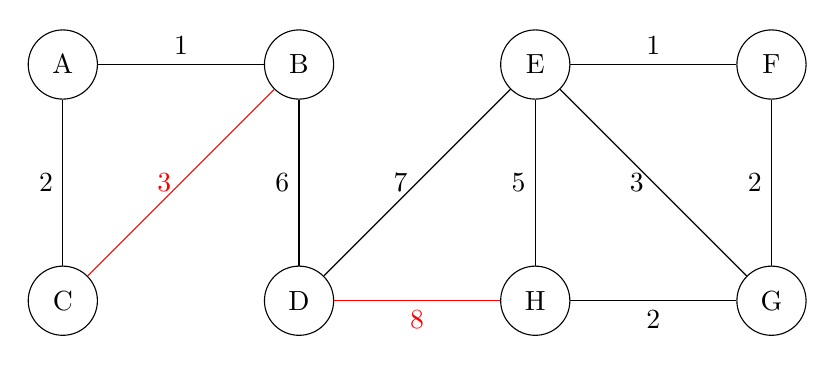
\begin{tikzpicture}
        \node[state](A) at (0,0)  {A};
        \node[state](B) at (3,0)  {B};
        \node[state](C) at (0,-3) {C};
        \node[state](D) at (3,-3) {D};
        \node[state](E) at (6,0)  {E};
        \node[state](F) at (9,0)  {F};
        \node[state](G) at (9,-3) {G};
        \node[state](H) at (6,-3) {H};
        \path
            (A) edge [-, above] node {1} (B)
                edge [-, left ] node {2} (C)
            (B)
                edge [-, left , color=red] node {3} (C)
                edge [-, left ] node {6} (D)
            (D)
                edge [-, left ] node {7} (E)
                edge [-, below, color=red] node {8} (H)
            (E)
                edge [-, above] node {1} (F)
                edge [-, left ] node {3} (G)
                edge [-, left ] node {5} (H)
            (F)
                edge [-, left ] node {2} (G)
            (G)
                edge [-, below] node {2} (H)
            ;
    \end{tikzpicture}
\end{frame}
\end{document}
